\begin{comment}
TODO:
--> Bildquellen überprüfen
--> Referenzen zu Bilder, Tabellen und Quellen im Text prüfen
--> Einarbeitungleitfaden ergänzen: neuer Knoten anlegen, Directory builden usw aus Fabis Anleitung
--> Einarbeitungleitfaden ergänzen: Midnight Commander 

--> Kapitel zur Fernsteuerung des EVObots: zuerst via VNC Client Desktop gespiegelt, um mobil ohne Bildschirm und Maus/Tastatur auf Gerät arbeiten zu können. Später hat sich aber gezeigt, dass Grafikberechnung und Übertragung des Desktops zu viel Rechenleistung benötigt, wodurch Rechenleistung von ROS reduziert wird, demnach kamen Algorithmen zum Spurhalten dem realen Verhalten nicht hinterher, deshalb Zeitverzug und keine Spurregelung möglich! Umstieg auf SSH zugriff via Terminal auf PC, grafische Benutzeroberfläche auf Ubuntu deaktiviert, um sämtliche Ressourcen für ROS zu generieren. Ergebnis zeigt echtzeitgetreue Spurerfassung und Regelung!

CAN-to-WiFi Gateway mit PaspberryPi oder Ardiuno möglich

Mehr Zustandsüberwachungssystem als Diagnosesystem 

Off-Board-Kommunikation als Diagnose in ISO Schicht 7 geregelt 

Generierung von Diagnosedaten ist von Beginn der Entwicklung an essentiell, um spätere Komplexität zu beherrschen. 

Fehler sind üblich in komplexen Systemen. Sollten vermieden werden, kommen aber unter bestimmten Bedingungen und Voraussetzungen vor. Abhängig von Implementierung, Fehlervermeidung usw. Fale-Safe-Zustand. Fehlerzustand, Fehlerwirkung
Wie äußert sich Fehler oder Fehlfunktion? --> unplausibler Signalwert, falscher Wert oder out of range

Abweichung zum SOLL ist nicht unbedingt programmseitiger Fehler, sondern kann aus Logikfunktion des Programmierers folgen. 
\end{comment}



\chapter{Diagnosesystem} \label{cha:Diagnosesystem}

Dieser Kapitel soll detailliert die zentrale Aufgabe der Arbeit beschreiben. Es solle Verfahren zu Diagnose des EVObots entwickelt und erstellt werden, um im Fahrbetrieb die internen Zustands- und Sensordaten echtzeitnah darzustellen und somit die Applikation des Fahralgorithmus zu erleichtern. 
Zunächst wird die Bedeutung der Diagnose eines komplexen Fahrzeugsystems mit vernetzten Systemen aufgezeigt und ein Konzept zur Fehlerdiagnose am Modellfahrzeug aufgebaut. Nachfolgend wird das Vorgehen und der Aufbau eines Diagnosesystems ausführlich beschrieben. Abschließend wird die Diagnosefunktion validiert und die gewonnen Ergebnisse betrachtet. 

\section{Konzept der Fehlerdiagnose} \label{sec:KonzeptDiagnose} % Allgemeines zur Diagnose im Fzg usw., Methodenauswahl: Warum CAN, Alternativen beschreiben (kabellos?), Use-Case-Diagramm

Aktuelle Fahrzeugsystemen sollten selbstredend stets fehlerfrei und ohne Probleme agieren und die vom Fahrer gewünschten Funktionen vollständig umsetzten. Trotzdem kann es unter gewissen Umständen und äußeren Voraussetzung zu einem Fehlverhalten kommen. Ein Fehler kann im Betrieb eines mechatronischen Systemverbund sowohl mechanisch, elektronisch, als auch softwareseitig auftreten. Durch den stetigen Anstieg des Softwareanteils und der sicherheitskritischen Prozesse im automotiven Bereich steigt die Gefahr eines Softwarefehlers oder einer Software-Anomalie. Ein Fehler wird dabei allgemein nach \emph{EN ISO 9000:2005} \cite{DINDeutschesInstitutfurNormunge.V..201511} als \glqq Nichterfüllung einer Anforderung\grqq{} oder nach \emph{DIN 55350} \cite{DINDeutschesInstitutfurNormunge.V..200805} genauer als \glqq eine unzulässige Abweichung eines Merkmals von einer vorgegebenen Forderung\grqq{} beschrieben. \\
Ein Softwarefehler lässt sich allgemeingültig entweder durch physikalische beziehungsweise chemische Effekte oder durch menschliche Fehlermechanismen wie Denkfehler, Verständnisfehler, Interpretationsfehler oder simple Tippfehler beschreiben. Dabei kann man diese Beschreibung eines Fehlers grundsätzlich in zwei Kategorien einordnen: Man spricht von einem physikalischen Fehler, wenn einzelne Komponenten oder Teilsysteme ausfallen, oder von einem funktionalen Fehler, wenn ein System ausführbar ist, seine Funktion aber nicht korrekt umgesetzt wird \cite{Borcsok.2007}. Ein funktionaler Fehler ist offenbar in den meisten Fällen das Ergebnis von Design-Mängeln und demnach auf eine menschliche Ursache zurückzuführen. Eine Fehlhandlung in der Umsetzung einer Softwareanwendung führt in aller Regel zu einem Fehlerzustand bei der Programmausführung. Dieser Fehlerzustand kann unter Umständen auch unerkannt bleiben. Tritt der Fehlerzustand jedoch aus Programmsicht nach Außen auf, spricht man von der Fehlerwirkung, die für den Anwender wahrnehmbar ist. Diese Fehlerwirkung kann sich je nach Schwere des Fehlers als ein abweichender Rückgabewert einer Berechnung oder bis hin zum Totalausfall des Systems äußern \cite{ISTQBAISBLGermanTestingBoarde.V.2017}. \\
Im Sinne der Zuverlässigkeit gilt es also, das Auftreten eines Fehlerzustandes in einem sicherheitskritischen System zu vermeiden oder besser einen sicheren Zustand im Fehlerfall einzunehmen. Ein übergeordnetes Beispiel eines \emph{Fail-Safe}-Zustandes kann aus der Technologie des hochautomatisierten Fahrens gegeben werden: Fällt das Kamerasystem zur Fahrspurerkennung unerwartet aus, soll ein automatisiert fahrendes Fahrzeug nicht unkontrolliert weiterfahren, sondern die Fahrgeschwindigkeit reduzieren und auf Basis der verfügbaren Streckendaten am rechten Fahrbahnrand zum Stehen kommen, um einen potentiellen Schaden zu minimieren.
 
Die Komplexität der vernetzten Funktionen und Systeme erfordert eine umfassende Kommunikation der Softwarekomponenten und ebenso ausgereifte Methoden zur Diagnose möglicher Fehler. Der Begriff \emph{Diagnose} stammt eigentlich aus der Medizin, lässt sich aber \cite{Reif.2014} nach im Bezug auf Fahrzeuge wie folgt definieren: \glqq Aus konkreten und diffusen Symptomen, die der Fahrer schildert, wird im Service unter Zuhilfenahme der Diagnosesysteme ein exaktes Fehlerbild erstellt und es werden geeignete Reparaturmaßnahmen eingeleitet.\grqq{} Der Ablauf einer klassischen Fehlerdiagnose lässt sich anhand dem Modell \ref{abb:AblaufDiagnose} veranschaulichen. 
\begin{figure}[!htbp]
	\centering
	\tikzstyle{block} = [rectangle, rounded corners, minimum width=4cm, minimum height=1cm, text centered, draw=black]
	\tikzstyle{ergebis} = [rectangle, rounded corners, minimum width=4cm, minimum height=1cm, text centered]
	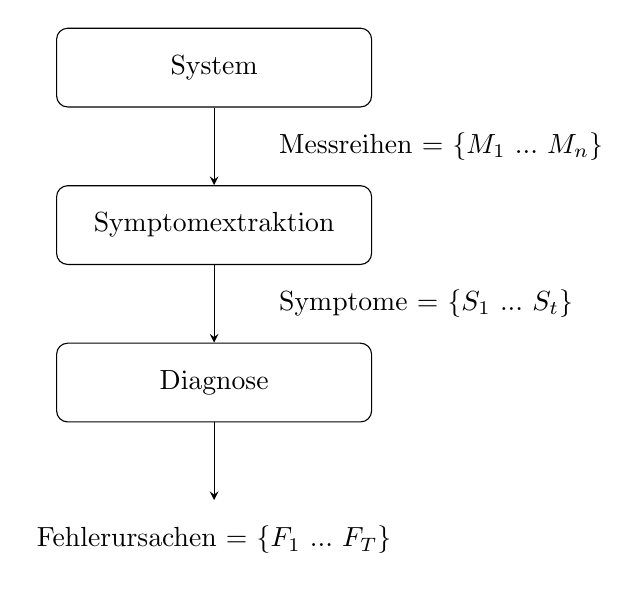
\begin{tikzpicture}[node distance=2cm]
	\node (system)   [block] {System};
	\node (symptom)  [block, below of=system] {Symptomextraktion};
	\node (diagnose) [block, below of=symptom] {Diagnose};
	\node (fehler) [ergebis, below of=diagnose] {Fehlerursachen = $\{F_1 ~...~ F_T\}$};
	
	\draw[->,>=stealth] (system)   -- node[anchor=west] {\qquad Messreihen = $\{M_1 ~...~ M_n\}$} (symptom);
	\draw[->,>=stealth] (symptom)  -- node[anchor=west] {\qquad Symptome = $\{S_1 ~...~ S_t\}$}   (diagnose);
	\draw[->,>=stealth] (diagnose) -- (fehler);
	\end{tikzpicture}
	\caption{Ablauf einer Diagnose im Kfz-Umfeld \cite{Leonhardt.1997}}
	\label{abb:AblaufDiagnose}
\end{figure}
Ein Diagnosesystem, welches mittels Symptome Fehlerursachen diagnostiziert, kann also formal als eine Abbildung von Fehlersymptomen S auf Fehlerursachen F angesehen werden
\begin{displaymath}
	\{S_1 ~...~ S_t\} \rightarrow \{F_1 ~...~ F_T\}.
\end{displaymath}

Kommt es zu einem Fehlerfall oder Systemausfall, ist die Ursache in einem komplexen und verteilten Systemnetzwerk meist schwer auszumachen. Aufgrund dessen wurden bereits früh in der Entwicklung elektronischer Datenkommunikation Diagnosesysteme als Analysewerkzeug eingeführt. Mit einem aus Hard- und Software bestehenden Diagnosesystem kann die Datenbuskommunikation aufgezeichnet und diagnoserelevante Informationen über den Zustand der Teilkomponenten zu einem externen Testgerät übertragen und ausgewertet werden. Ein Diagnosesystem gilt damit als umfangreiches Werkzeug zur schnellen Fehlererkennung und Fehleranalyse. Während dem Entwicklungsprozess lässt sich ein Diagnosesystem auch nutzen, um über die Diagnosekommunikation die Steuergeräte-Applikation durchzuführen. Dabei ist es nicht nur nötig die reine Datenübertragung einheitlich zu standardisieren, sondern ebenfalls die Applikationsschicht der Protokolle (Vgl. Tabelle \ref{tab:OSI-Schichtenmodell}) zu normieren. Dies bietet die Möglichkeit, den Aufwand und die Pflege der Diagnoseschnittstellen und den Diagnosetestern zu begrenzen. \\
Um eine einheitliche Diagnosekommunikation zu schaffen, wurden seit den 1990er Jahren diverse \emph{Diagnoseprotokolle} entwickelt, die zunächst teils proprietär und inkompatibel zueinander umgesetzt waren, inzwischen jedoch meist herstellerübergreifend genormt sind. Als heute gängige Diagnoseprotokolle sind das \emph{Keyword 2000 Protokoll} \acs{KWP} 2000, die \emph{Unified Diagnostic Services} \acs{UDS} oder die \emph{On-Board-Diagnose} \acs{OBD} zu nennen. Für weiterführende Informationen der genannten Standards sei auf \cite{Zimmermann.2014} und \cite{Schaffer.2012} verwiesen. Die verschiedenen Protokolle einer Diagnosekommunikation lassen sich auf die einzelnen Schichten des bekannten ISO/OSI-Referenzmodells anwenden. Das eigentliche Diagnoseprotokoll umfasst dabei abhängig von seiner Ausprägung und dem expliziten Anwendungsfall die Schichten fünf bis sieben. Die Übertragung der Diagnosedaten erfolgt durch entsprechende Protokolle für das angewendete physikalische Kommunikationsmedium in den Schichten eins bis vier. 


\subsection{Anforderungen an die Fehlerdiagnose}
\label{subsec:AnforderungenDiagnose}

Um ein Diagnosesystem für das Demonstratorfahrzeug mit angemessenen Mitteln und Werkzeugen umzusetzen, wird zunächst der gewünschte Funktionsumfang beschrieben und darauf aufbauend sämtliche Anforderungen an das System definiert.
Dazu ist in Abbildung \ref{abb:UseCaseDiagnose} ein Use-Case-Diagramm in der grafischen Modellierungssprache \acs{UML} für den konkreten Anwendungsfall der Diagnosefunktion dargestellt. Hieraus lassen sich leicht die Spezifikationen und geforderte Funktionalitäten an die spätere Diagnose ableiten.

\begin{figure}[!htb]
	\centering
	\begin{tikzpicture}
	\tikzumlset{fill usecase=gray!20}
	\begin{umlsystem}[x=4]{Diagnosefunktion} 
	\umlusecase [x=0.5, y=0,    width=2.5cm] {Diagnose starten/stoppen}
	\umlusecase [x=0,   y=-2,   width=2.5cm] {Diagnosedaten aufzeichnen}
	\umlusecase [x=0.5, y=-4,   width=2.5cm] {Diagnosedaten ausgeben}
	\umlusecase [x=0,   y=-6,   width=2.5cm] {in Klartext darstellen}
	\umlusecase [x=4,   y=-7.5, width=2.5cm] {Signalverlauf darstellen}
	\umlusecase [x=5,   y=-3,   width=2.5cm] {Daten einlesen}
	\umlusecase [x=5.5, y=-1,   width=2.5cm] {Sensordaten einlesen}
	\umlusecase [x=5.5, y=-5,   width=2.5cm] {statische Daten einlesen}
	\end{umlsystem}
	
	\umlactor [y=-2] {Anwender}
	\umlactor [x=13, y=-3] {EVObot}
	
	\umlassoc{Anwender}{usecase-1}
	\umlassoc{Anwender}{usecase-2}
	\umlassoc{Anwender}{usecase-3}
	\umlassoc{EVObot}{usecase-6}
	\umlinherit{usecase-4}{usecase-3}
	\umlinherit{usecase-5}{usecase-3}
	\umlinherit{usecase-7}{usecase-6}
	\umlinherit{usecase-8}{usecase-6}
	\umlextend{usecase-6}{usecase-1} 
	
	\end{tikzpicture}
	\caption{Use-Case-Diagramm einer Diagnosefunktion für den Fahrdemonstrator}
	\label{abb:UseCaseDiagnose}
\end{figure}
	
Das Gesamtsystem besteht aus Fahrzeug, Diagnosewerkzeug und Anwender. Aus dem Use-Case-Diagramm ergeben sich die funktionalen Anforderungen wie folgt:

\begin{itemize}
	\item Das Diagnosesystem muss die Diagnosedaten innerhalb der Programmlaufzeit an ein Ausgabegerät übermitteln.
	\item Das Diagnosesystem muss die Diagnosedaten auf einem externen Ausgabegerät darstellen.
	\item Das Diagnosesystem muss die Daten sowohl in Klartext ausgeben, als auch die einzelnen Signalverläufe grafisch darstellen. 
	\item Die Diagnosefunktion muss vom Anwender gestartet und gestoppt werden können.
	\item Das Diagnosesystem darf im inaktiven Zustand keine Daten vom Fahrzeug übertragen, um die Systemauslastung gering zu halten.\\
\end{itemize}


Weiterhin lassen sich folgende, nichtfunktionale Anforderungen stellen:
\begin{itemize}
	\item Die Umsetzung der Datenkommunikation soll dem Vorbild eines realen und aktuellen Kraftfahrzeuges entsprechen.
	\item Die Datenkommunikation darf kabelgebunden oder kabellos stattfinden.
	\item Das Diagnosesystem muss ein echtzeitnahes Daten-Monitoring ermöglichen.
	\item Das Diagnosesystem soll eine übersichtliche Visualisierung für den Anwender bieten. 
	\item Die Einbindung in das bestehende System soll ohne grundlegende Modifikationen in den implementierten Algorithmen möglich sein.
	\item Die Datenkonsistenz und Datensicherung bei der externen Kommunikation muss gewährleistet sein.
	\item Die Diagnosefunktion muss für spätere Ergänzungen erweiterbar sein.
	\item Die Programmierschnittstelle muss offen und modular sein. 
\end{itemize}

% Echtzeitnah, Livebeurteilung und Aufzeichnung möglich, visuell gut umsetzbar, Aufwand überschaubar, Einbindung in bestehendes System nur durch Erweiterung, vergleichbare Umsetzung wie im Kfz, Datenkonsistenz und Zuverlässigkeit (Sicherheitsaspekte von CAN), kabellos oder kabelgebunden (keine langen Fahrwege), leichte Erweiterung 

\subsection{Möglichkeiten zur Umsetzung einer Fehlerdiagnose}
\label{subsec:MöglichkeitenDiagnose}

Die Umsetzung einer Diagnosefunktion und die Einbindung dieser Funktion in das Gesamtsystem auf dem Betriebssystem des Demonstratorfahrzeuges lässt sich grundsätzlich mit verschiedenen Mitteln und Möglichkeiten erzielen. Die bedingt voneinander entkoppelten Teilfunktionen umfassen:
\begin{itemize}
	\item Sammeln der Sensordaten und Nutzinformationen im Gesamtsystem von ROS.
	\item Bereitstellung dieser Daten in einer zur Übertragung geeigneten Form.
	\item Echtzeitnahe Übermittlung der Diagnosedaten an ein externes Ausgabegerät.
	\item Analyse und Visualisierung der Daten auf dem Ausgabegerät. 
\end{itemize}

Ein Ansatz zur möglichen Umsetzung besteht darin, sämtliche im bereits implementierten Quelltext des Software-Framework ROS berechneten und vorhandenen Wertevariablen und Sensordaten während der Programmlaufzeit drahtlos durch ein lokales Netzwerk zu übermitteln. Hierzu eignen sich diverse Industriestandards für Funknetzwerke nach \emph{\acs{IEEE} 802} wie Bluetooth oder WLAN. Ein großer Vorteil der Bluetooth-Technologie liegt in dem Verbindungsaufbau der Kommunikationspartner. Die Bluetooth-Knoten müssen sich lediglich in Reichweite befinden, um eine automatische Verbindung aufzubauen, ohne, dass eine Anwenderinteraktion nötig wird. Damit eignet sich Bluetooth für einen Datenaustausch mit autonomen Systemen. Um eine mögliche Bluetooth-Verbindung mit dem \emph{NVIDIA Jetson}-Modul aufzubauen, ist lediglich ein geeigneter Bluetooth-Adapter nötig. Die Bluetooth-Technologie eignet sich zwar für eine einfache, drahtlose Punkt-zu-Punkt-Datenkommunikation und weist eine allgemeine Reichweite von circa 10 Metern auf, die Reichweite ist jedoch stark abhängig von der Sendeleistung und der Empfindlichkeit des eingesetzten Transceivers. Zusätzlich können die Eigenschaften der Umgebung die erzielbare Sende- und Empfangsreichweite negativ beeinflussen, wodurch eine konsistente Datenverbindung je nach Einsatzumgebung des Fahrdemonstrators nicht gewährleistet ist.
Kommt es bei einer Datenverbindung auf hohe Übertragungsraten und erhöhte Sicherheit an, eignet sich eher die Verbindung durch WLAN in einem drahtlosen lokalen Netzwerk. Diese Übertragung ist jedoch explizit an einen stationären Ort gebunden. Fällt das Netzwerk aus, kann also keine Datenkommunikation stattfinden. Zudem ist die Latenz bei einer WLAN-Verbindung nicht kontrollierbar und kann unter Umständen so hoch sein, dass eine Echtzeitanwendung nur mit erhöhtem Aufwand umsetzbar ist. \\
Um dem zentralen Anspruch gerecht zu werden, die Datenkommunikation vergleichbar zu der eines realen Fahrzeuges aufzubauen, liegt es nahe, den Datenaustausch zwischen dem Fahrzeug und einem externen Ausgabegerät durch ein in der Fahrzeugtechnik übliches serielles Bussystem zu realisieren. Hierzu eignet sich vor allem das CAN-Protokoll, das durch seine relativ hohen Datenraten, das deterministische Verhalten, eine fehlertolerante Datenübertragung und die robusten Datensicherungsmaßnahmen als die am häufigsten im Kfz eingesetzte serielle Kommunikationstechnologie gilt. Ein weiterer Aspekt, der für eine Verwendung des CAN-Protokolls spricht, ist das bereits vorhandene Vorwissen zu Bussystemen und die Verfügbarkeit sämtlicher nötiger Tools und Anwendungen im Unternehmen. Da sowohl diverse CAN-Interfaces, als auch die nötigen Softwarelizenzen unternehmensintern zur Verfügung stehen, wird die Realisierung der Diagnosefunktionalität mit einem seriellen Bussystem als besonders geeignet betrachtet. 
Daher wird der Ansatz verfolgt, eine drahtgebundene Off-Board-Kommunikation über eine physikalische Busleitung zwischen dem Fahrzeug und einem externen Laptop aufzubauen, um die Fahrzeugzustandsdaten online\footnote{Als \emph{online} wird hier nicht die aktive Verbindung zum Internet bezeichnet, sondern die intakte und betriebsbereite Datenverbindung zwischen EVObot und dem externen Ausgabegerät.} im Fahrbetrieb zu analysieren und eine Datenaufzeichnung zu ermöglichen. Die Menge der zu übermittelnden Diagnosedaten hängt dabei selbstredend von der Komplexität der umgesetzten Funktionalitäten und der verwendeten Sensorik des autonomen mobilen Roboters ab. Nach einer ersten Sichtung der implementierten Algorithmik kann bereits festgehalten werden, dass eine Übertragung größerer, zusammenhängender Datenmengen nicht nötig ist. Es genügt, die internen Zustands- und Sensordaten in Form einzelner Signale gebündelt in zyklischen Busbotschaften zu übermitteln. Eine Segmentierung der Datenmengen, wie es bei einem \emph{Transportprotokoll} in Kfz-Anwendungen auf der Transportschicht im ISO/OSI-Schichtenmodell (vgl. Tabelle \ref{tab:OSI-Schichtenmodell}) üblich ist, wird daher nicht nötig sein. Aufgrund dessen wird bei Implementierung der Diagnosefunktion bewusst auf die Umsetzung der Schicht vier des Referenzmodells verzichtet.
Der Verzicht auf die Verwendung eines normierten Transportprotokolls impliziert eine weitere Einschränkung des Diagnosesystems: Üblicherweise werden im Fahrzeugbetrieb erkannte Fehlfunktionen und Störungen durch einen Eintrag im Fehlerspeicher des Steuergerätes dokumentiert. Diese Einträge weisen neben den nach dem Diagnoseprotokoll normierten Fehlercodes und einer Fehlerbeschreibung zusätzliche situationsabhängige Umgebungsdaten und zeitliche Informationen auf. Da die zu implementierende Diagnosefunktion lediglich ein echtzeitnahes Daten-Monitoring ermöglichen soll und eine Speicherung, respektive  Auswertung der Diagnosedaten nur auf dem externen Diagnoserechner nötig ist, wird im weiteren Verlauf auf die formale Definition eines Fehlerspeichers und der Regeln zur Fehlerablage verzichtet. Demzufolge steht die strikte Einhaltung des standardisierten Datenmodells für den Austausch diagnoserelevanter Daten nach dem \emph{Open Diagnostic Data Exchange} \acs{ODX}-Standard nicht im Fokus der Arbeit.


\section{Aufbau einer Datenkommunikation auf CAN-Bus} \label{sec:AufbauDatenkommunikation} % HW-Anbindung an CAN-Bus, Arduino/Jetson, Darstellung Übertragung Dummy-Botschaften cansend/candump, MTTCAN Treiber Kernel rebuild, Socketcan erklären, python-can, can-utils
Neben der softwareseitigen Umsetzung einer Datenkommunikation spielt die physikalische Busanbindung auf dem EVObot entsprechend der Bitübertragungsschicht im ISO/OSI-Schichtenmodell eine zentrale Rolle. 

\subsection{Fahrzeugseitige Busanbindung} \label{subsec:FahrzeugseitigeBusanbindung}
Zur Übertragung einzelner CAN-Botschaften vom Modellfahrzeug auf einen externen Diagnoserechner stehen mehrere Möglichkeiten zur Auswahl. Zum einen lässt sich die Hardwareanbindung über einen Arduino realisieren. Auf dem EVObot ist bereits ein Arduino Uno verbaut, der das Eingangssignal des Ultraschallsensors einliest und zum Ansteuern der Aktorik eingesetzt wird. Durch die Erweiterung des Arduinos um ein \emph{CAN-Bus Shield} lässt sich ein feldbusfähiges Kommunikationssystem aufbauen. Ein CAN-Shield erweitert den herkömmlichen Mikroprozessor der Arduino-Plattform um einen CAN-Controller mit einer SPI-Schnittstelle und einem geeigneten CAN-Transceiver. Die verfügbaren CAN-Bus Shields implementieren den üblichen CAN High Speed Standard mit einer maximalen Datenrate von 1\,Mbit/s, was die Anforderungen an die  Datenübertragung in der späteren Verwendung in jedem Fall erfüllt. Es können Identifier sowohl im 11\,Bit Standard-Format, als auch im 29\,Bit Extended-Format verarbeitet werden. Zudem liefert eine solche Erweiterungsplatine umfangreiche Programmbibliotheken, um die Verwendung einer CAN-Anbindung in der Arduino Entwicklungsumgebung zu ermöglichen. Es lassen sich sämtliche diagnoserelevante Daten von dem Hauptrechner, dem NVIDIA Jetson TX2, über die serielle Schnittstelle zyklisch an den Arduino senden. Auf diesem werden die Informationen in das gängige CAN-Format gepackt und physikalisch auf den Bus gesendet. Da es jedoch ein explizites Projektziel ist, künftig auf die Verwendung des Arduinos zu verzichten, wäre es nicht zielführend, die Diagnosekommunikation hardwareseitig durch einen Arduino mit einem Erweiterungsboard zu realisieren.

Aufgrund dessen wird die Busanbindung direkt über das NVIDA Jetson TX2 realisiert. Dieses bietet gegenüber dem Vorgängermodell Jetson TX1 den entscheidenden Vorteil, bereits ein CAN-Interface mit zwei Controllern auf dem Mainboard verbaut zu haben. Dadurch kann die Busanbindung direkt auf dem Board umgesetzt werden, sodass kein Routing der Busbotschaften über einen Arduino nötig wird. Das interne Interface unterstützt ebenfalls übliche Datenraten bis zu 1\,MBit/s und ist sowohl für Identifier im Standard-Format, als auch im Extended-Format ausgelegt. Abbildung \ref{abb:JetsonTX2CANConnector_BW} ist die Anschlussbelegung der CAN Architektureinheit des Tegra-Chips auf dem Jetson TX2 zu entnehmen. Es sind je eine Sendeleitung (\emph{Tx}) und eine Empfangsleitung (\emph{Rx}) dargestellt. Damit lässt sich ein Netzwerk mit zwei unabhängigen Busleistungen implementieren. Darüber hinaus bietet die Architektur eine Einbindung von Fehlerdetektionsleitungen zur Sicherstellung netzweiter Datenkonsistenz und weitere Signalleitungen für abstraktere Busanwendungen.

\begin{figure}[!htbp]
	\centering
	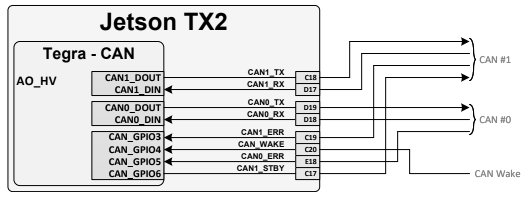
\includegraphics[width=12cm]{./Jetson_TX2_CAN_Connector_BW}
	\caption{Layout des CAN-Interfaces auf dem NVIDIA Jetson TX2 nach dem NVIDIA Product Design Guide \cite{NVIDIACorporation.2017}}
	\label{abb:JetsonTX2CANConnector_BW}
\end{figure}

Das Jetson TX2 verfügt zwar über einen integrierten Controller, um eine Busbotschaft physikalisch zu versenden oder empfangen und korrekt zu interpretieren, ist jedoch zusätzlich ein externer CAN-Transceiver nötig. Der CAN-Controller wickelt das Protokoll ab, während der Transceiver die physikalische Verbindung zu CANH und CANL darstellt. Möchte ein CAN-Knoten auf den Bus senden, erhält der Transceiver die Businformationen vom $\mu$C über den Controller (vgl. Abbildung \ref{abb:CANNetzwerk}). Der Transceiver setzt die empfangenen Daten in einen Spannungspegel um, sodass ein differentielles Spannungssignal auf die Busleitung gesendet wird. Beim Empfangen wandelt er die Spannungspegel dagegen in für den Controller verwertbare Signale um.\\
Nach einer Recherche zu geeigneten CAN-Transceivern fiel die Entscheidung auf das Modell \emph{SN65HVD230} der Firma \emph{Texas Instruments Incorporated}. Ein Auszug des frei verfügbaren Datenblattes ist Anhang \ref{app:anhang_1} zu entnehmen. Dieser Transceiver ist bereits auf einem Breakout Board der Firma \emph{Waveshare} montiert und als Steckmodul verfügbar. Zur Spannungsversorgung des Transceivers sind 3,3\,V nötig, die über einen GPIO-Port des Jetson TX2 abgegriffen werden können. Die CANH- und CANL-Leitungen können mit einer Schraubklemme mit dem Steckmodul verbunden werden. Der Transceiver wird wie in Abbildung \ref{abb:AnschlussbelegungTransceiver} dargestellt mit dem Jetson-Board an der GPIO-Steckleiste J26 verbunden. Zusätzlich werden zwei LEDs angekoppelt, um das Senden und Empfangen von CAN-Botschaften zu visualisieren.

\begin{figure}[!htbp]
	\centering
	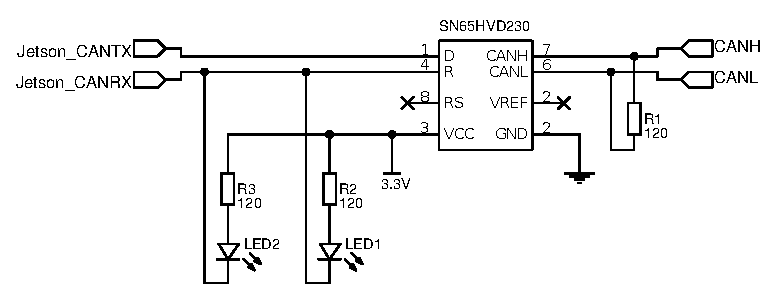
\includegraphics[width=12cm]{./CAN_Transceiver_Schematic_pdf}
	\caption{Schaltplan des SN65HVD230 CAN-Transceivers}
	\label{abb:AnschlussbelegungTransceiver}
\end{figure}

Um CAN-Botschaften über das Jetson TX2 zu versenden, sind zunächst einige grundlegende Einstellungen und Änderungen im Betriebssystem vorzunehmen. An erster Stelle muss  ein geeigneter Treiber installiert und aktiviert werden, der das CAN-Interface unterstützt. Hierfür kommt das Modul \emph{MTTCAN} der Firma \emph{Robert Bosch GmbH} zum Einsatz. Der Treiber legt die Konfiguration der logischen Verschaltung auf dem Mikroprozessor des Jetson TX2 fest und ermöglicht damit die protokollkonforme Verarbeitung der Datenübertragung über CAN-Bus. Es lassen sich empfangene Busnachrichten filtern und nach ihrer Priorität sortieren, um dadurch die Interrupt-Last zu reduzieren. Nach einem Rebuild des Kernels und einem Hinzufügen des Kernelmoduls zur Laufzeit des Systems ist der Treiber aktiv. Bei der Überprüfung der Systemkonfiguration werden nun beide CAN-Controller als korrekt konfiguriert gelistet.\\
Um mit der CAN-Konfiguration auf dem Jetson TX2 arbeiten zu können, wird die generische Programmierschnittstelle \emph{SocketCAN} eingesetzt. Diese \acs{API} stellt eine Sammlung von diversen Netzwerktreibern und einer eigenen Netzwerkschicht, die ursprünglich von der Konzernforschung der \emph{Volkswagen AG} als Open Source Projekt für die Verwendung von CAN unter Linux entwickelt wurde. Es beinhaltet dabei Treiber zum Aufbau verschiedener Schnittstellen als Sockets und lehnt sich somit an das \emph{TCP/IP}-Protokoll an, das zur Netzwerkprogrammierung verwendet wird. SocketCAN erzeugt ein neues virtuelles Netzwerkgerät auf dem Betriebssystem und ermöglicht damit, mehreren Anwendungen gleichzeitig auf CAN-Funktionen zugreifen zu können. Es können ebenfalls mehrere CAN-Netzwerke von einzelnen Anwendungen parallel genutzt werden. Damit bietet SocketCAN eine benutzerfreundliche Umsetzung des zyklischen Versenden von Diagnosebotschaften auf dem CAN-Bus. Zusätzlich liefert die offene Programmierschnittstelle flexible Erweiterungen zum Einsatz von Transportprotokollen um auch größere Datenmengen segmentiert auf einzelne Busbotschaften versenden zu können. Dies wird jedoch wie bereits in Abschnitt \ref{subsec:MöglichkeitenDiagnose} erläutert aufgrund der begrenzten Anzahl der Zustands- und Sensordaten für die gewünschte Anwendung nicht nötig. Ein Mehrwert für die Diagnosefunktion bietet jedoch der Broadcast-Manager von SocketCAN. Dieser ermöglicht CAN-Botschaften zu filtern und periodisch zu verschicken \cite{OliverHartkopp.2017}.
Um CAN-Botschaften letztlich durch Kommandozeilenbefehle versenden und analysieren zu können und um das zunächst rudimentäre Busnetzwerk zu testen, kommt das Linux-Tool \emph{can-utils} zum Einsatz. Einige verwendete Befehlsanwendungen, die das Dienstprogramm liefert, sind:

\renewcommand{\arraystretch}{1.5}
\begin{tabular}{l l}
	\texttt{\textbf{cansend}}: & Senden einer Single Frame Botschaft\\
	\texttt{\textbf{cangen}}: & Erzeugen von zufälligem CAN-Busverkehr\\
	\texttt{\textbf{canplayer}}: & Wiedergabe von CAN-Logfiles\\
	\texttt{\textbf{candump}}: & Anzeigen, Filtern und Protokollieren von CAN-Botschaften\\
	\texttt{\textbf{cansniffer}}: & Anzeige inhaltlicher Unterschieder zweier CAN-Botschaften\\
	\texttt{\textbf{canbusload}}: & Berechnen und Anzeigen der Buslast
\end{tabular}

Um die Konfiguration des Bussystemes zu testen, werden die beiden internen CAN-Controller des Jetson TX2 als Busknoten gesetzt. Wie in Abbildung \ref{abb:AnschlussbelegungTransceiver} werden zwei Transceiver an die entsprechenden GPIO-Pins für CAN\_TX und CAN\_RX des Jetson TX2 angeschlossen und über eine verdrillte Zweidrahtleistung miteinander verbunden. Dieser Aufbau entspricht nun einem vollständigen CAN-Netzwerk mit zwei sende- und leseberechtigten CAN-Knoten.
Als letzter Schritt muss die gewünschte Datenrate konfiguriert und die Netzwerkschnittstellen aktiviert werden. Dies wird mit dem Befehl 
 
	\begin{verbatim}
	nvidia@tegra-ubuntu:~$ ip link set can0 type can bitrate 500000
	                       ip link set up can0
	                       ip link set can1 type can bitrate 500000
	                       ip link set up can1
	\end{verbatim}

durchgeführt. Die Datenübertragungsrate muss für alle CAN-Knoten im selben Netzwerk übereinstimmen, um eine synchrone und fehlerfreie Datenübertragung zu gewährleisten. In der Fahrzeugindustrie hat sich bei CAN-Bussystemen eine Datenrate von typischerweise 500\,kBit/s etabliert, weshalb auch hier diese Verwendung findet.\\
Werden nun durch den Befehl \texttt{cangen can0} Busbotschaften des Knoten CAN0 generiert, können diese Botschaften auf dem Interface CAN1 empfangen und ausgelesen werden:

\begin{addmargin}[1cm]{0cm} 
\begin{verbatim}
nvidia@tegra-ubuntu:~$ candump can1
    can1   715   [1]   A6
    can1   4D0   [8]   43 44 AB 7B A6 62 01 1B
    can1   2B6   [2]   98 16
    can1   4C1   [8]   BE 3B 0F 36 72 40 CC 72
    can1   0DB   [4]   93 B8 5E 76
    can1   714   [5]   A8 A0 AB 78 A3
    can1   730   [1]   82
    can1   049   [8]   C7 44 D5 51 5E 07 27 75
    can1   58A   [8]   E7 C1 80 3B 5A 1A 0C 4F
    can1   509   [8]   01 7D 0D 6A BF 8F 38 5A
    can1   5CC   [8]   B3 74 A5 7D 8D FA 8A 41
    can1   405   [1]   FF

\end{verbatim}
\end{addmargin}

Dabei gilt zu beachten, dass hier lediglich zufällige Botschaften mit zufälligen IDs erstellt und versendet wurden. Der Inhalt der Botschaften hat für die weitere Umsetzung keinerlei Bedeutung und soll lediglich das korrekte Versenden und Empfangen von Busbotschaften über die physikalische Busleitung darstellen.\\
Es sei hier noch angemerkt, dass es sich bei den \emph{can-utils}-Funktionen um Terminal-Anwendungen handelt, d.h. die einzelnen Befehle werden unter Linux im Terminal aufgerufen und die zugehörigen Funktionsparameter wie ID oder Botschaftsdaten als Kommandozeilenbefehl angegeben. Zur Realisierung der Diagnosefunktion wird von diesem Konzept abgewichen, um den Diagnoseumfang erweiterbar zu implementieren.


\subsection{Empfängerseitige Busanbindung} \label{subsec:EmpfängerseitigeBusanbindung}
Nachdem die Busanbindung aufgebaut und getestet wurde, muss nun der Laptop an die Busleitung gekoppelt und zum zyklischen Empfang der Diagnosedaten konfiguriert werden. Die gesamte Busverbindung wird wie in Abbildung \ref{abb:AufbauBuskommunikation} dargestellt aufgebaut. 

\begin{figure}[!htbp]
	\centering
	\tikzstyle{block1} = [rectangle, rounded corners, text width=4cm, minimum height=3cm, text centered, draw=black, fill=white]
	\tikzstyle{block2} = [rectangle, rounded corners, text width=5cm, text height=4cm, text centered, draw=black, fill=gray!20]
	\tikzstyle{block3} = [rectangle, rounded corners, text width=3cm, minimum height=2cm, text centered, draw=black, fill=gray!20]
	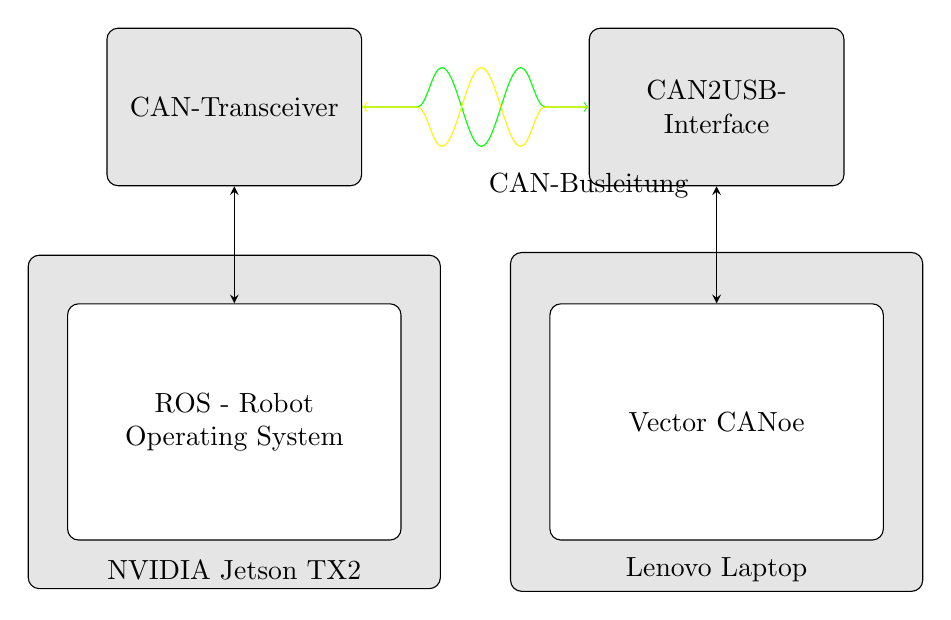
\begin{tikzpicture}
	\node (jetson)      [block2] at (0,0) {NVIDIA Jetson TX2};
	\node (ROS) 	    [block1] at (0,0) {ROS - Robot \\ Operating System};
	\node (transceiver) [block3] at (0,4) {CAN-Transceiver};
	\node (interface)   [block3] at (\textwidth-6cm,4) {CAN2USB-Interface};
	\node (laptop)      [block2] at (\textwidth-6cm,0) {Lenovo Laptop};
	\node (CANoe) 	    [block1] at (\textwidth-6cm,0) {Vector CANoe};
	\node (bus) at (4.5, 3) {CAN-Busleitung};
	
	\draw [<->,>=stealth] (ROS) -- (transceiver);
	\draw [<->,>=stealth] (interface) -- (CANoe);
	
	\draw [->, decorate, decoration ={snake, amplitude =.5cm, segment length =1cm, pre length=.7cm, post length=.5cm}, color=green](transceiver) -- (interface);
	\draw [<-, decorate, decoration ={snake, amplitude =-.5cm, segment length =1cm, pre length=.7cm, post length=.5cm},color=yellow](transceiver) -- (interface);

	\end{tikzpicture}
	\caption{Schematischer Aufbau der Buskommunikation zwischen dem EVObot und dem Diagnoserechner}
	\label{abb:AufbauBuskommunikation}
\end{figure}

Um die Buspegel auf der Empfängerseite von einer Differenzspannungssignal wieder in eine logische Signalfolge zu interpretieren, ist ein Interface nötig, welches das CAN-Protokoll auf einen universellen seriellen Bus umsetzt. Das \emph{CANcaseXL} der Firma \emph{Vector Informatik GmbH} ist ein USB-Interface, das eine physikalische Ankopplung eines Computers an ein reales Bussystem erlaubt. Mithilfe dieser Umsetzung ist es möglich, sowohl Busbotschaften zu generieren und diese auf den Bus zu senden, als auch reale Botschaften von angekoppelten Systemen auszulesen und auszuwerten. Über die beiden D-Sub DE9 Anschlüsse ist eine Verbindung zu \acs{CAN}- oder \acs{LIN}-Netzwerken realisierbar. Zwar wurde das CANcaseXL inzwischen von neueren Modulen abgelöst und bietet lediglich einen eingeschränkten Funktionsumfang gegenüber der weiteren Produktpalette der \emph{Vector Informatik GmbH}, jedoch eignet es sich aufgrund der vergleichsweise kompakten Bauform besonders für die hier gewünschte Anwendung. Zudem ist der integrierte Funktionsumfang für den Einsatz als \acs{CAN}-Interface völlig ausreichend \cite{VectorInformatikGmbH.2015}.

Zur softwareseitigen Auswertung und zum Versenden der Busbotschaften kommt das Software-Werkzeug \emph{CANoe} der Firma \emph{Vector Informatik GmbH} zum Einsatz. Das vielseitige Tool bedient Anwendungsgebiete wie Analyse, Diagnose, Simulation, Stimulation und Test während dem gesamten Entwicklungsprozess von Steuergeräten und Netzwerken. CANoe unterstützt dabei sämtliche gängigen Bussysteme sowie die normierten Transport- und Diagnoseprotokolle. Neben der Überwachung des realen Busverkehrs bietet die Software die Möglichkeit, einfache Teilsysteme bis hin zu komplexen Restbussystemen zu simulieren. Dabei kann die Buskommunikation jederzeit textuell dargestellt und die Signale visuell veranschaulicht werden \cite{VectorInformatikGmbH.2018}.\\
Das Softwaretool liefert zusätzlich die integrierte und firmeneigene Programmiersprache \emph{Communication Access Programming Language} \acs{CAPL}. Die auf \emph{C} basierte Sprache wurde speziell für die Anforderungen zur Entwicklung von Bussystemen angepasst. \acs{CAPL} bietet als eventorientierte Skriptsprache die Möglichkeit, bequem auf Signale zuzugreifen und die Signalwerte zu verändern. Es steht eine Vielzahl an vordefinierter Funktionen zur Verfügung. Ebenso können eigene grafische Benutzeroberflächen erstellt werden, wodurch komplexe Simulationsumgebungen erleichtert werden \cite{VectorInformatikGmbH.07.08.2017}. 


\section{Implementierung der Diagnosefunktion} \label{sec:ImplementierungDiagnose} % SW-seitige Umsetzung inkl. kompletter Programmablaufplan, Funktionen erklären, Gesamtfunktion in ROS, ... 

Nachdem nun alle hardwareseitigen Voraussetzungen erfüllt und sowohl der EVObot, als auch der Diagnoselaptop für eine Buskommunikation konfiguriert sind, kann die vollständige Diagnosefunktion implementiert werden. Es soll das Vorgehen bei der softwareseitigen Umsetzung beschrieben und relevante Auszüge aus Programmcode näher betrachtet werden.\\
Wie bereits in Abschnitt \ref{sec:EVObotSoftware} beschrieben, stellt das Framework Robot Operating System die zentrale Entwicklungsumgebung des Projektes dar. Daher kann auch aus den definierten Anforderungen der Anspruch entnommen werden, die Diagnose ebenfalls in ROS einzubinden. Dazu wird ein neuer Knoten\footnote{Der Begriff Knoten beschreibt in ROS in den meisten Fällen entkoppelt ausführbare Skripte, in denen diverse Funktionen umgesetzt werden. Daher wird nachfolgend im direkten Bezug zur ROS-Umgebung nicht zwischen den Begrifflichkeiten Diagnosefunktion und Diagnoseknoten unterschieden.} erstellt, der sich in die Knotenstruktur des ROS Entwicklungsprojektes eingliedert. Der bisherige Programmgraph wird aus Abbildung \ref{abb:rosgraphOhneDiagnose} ersichtlich.

\begin{figure}[!htbp]
	\centering
	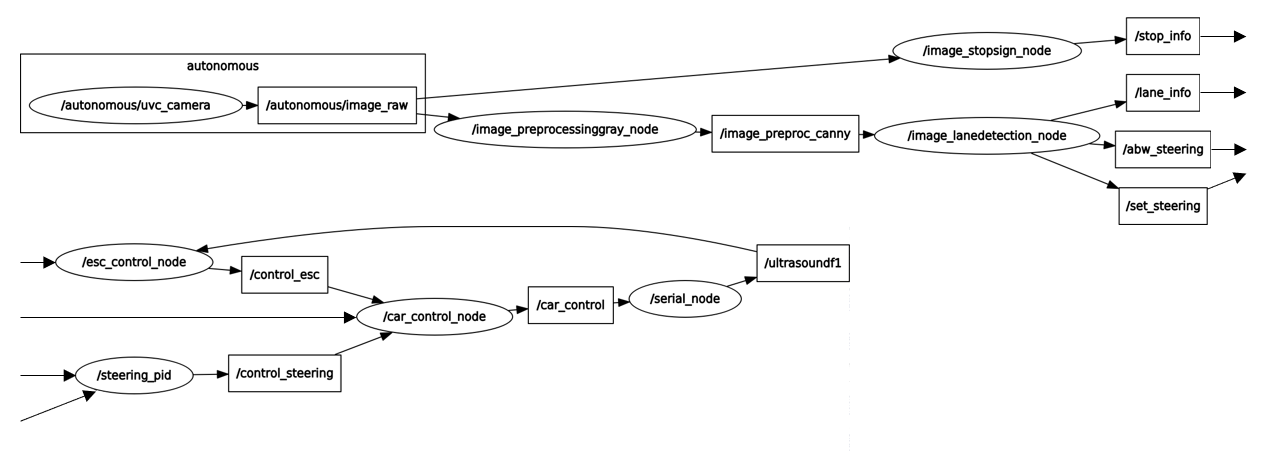
\includegraphics[width=\textwidth]{./rosgraph_ohne_diagnose_geteilt}
	\caption{Programmgraph des initialen ROS-Paketes \emph{autonomous}, mit dem Befehl \texttt{rqt\_graph} automatisch generiert}
	\label{abb:rosgraphOhneDiagnose}
\end{figure} 

Wie zuvor in Abschnitt \ref{sec:EVObotSoftware} erwähnt, werden Knoten in der ROS-Umgebung als ovale Felder dargestellt. Tauschen einzelne Knoten Informationen in Form von Messages aus, wird dies über die Topics genannten Datenstreams realisiert. Topics werden im Schaubild als Rechtecke dargestellt. Es sei an dieser Stelle angemerkt, dass die Darstellung in Abbildung \ref{abb:rosgraphOhneDiagnose} für eine angenehme Übersicht auf zwei Zeilen aufgeteilt wurde. Auf die expliziten Funktionsumfänge der einzelnen Knoten wird an späterer Stelle eingegangen.\\
ROS lässt sich sowohl in der sehr effiziente und maschinennahe Programmiersprache C++, als auch in der benutzerfreundlichen und universellen Skriptsprache Python betreiben. Python bietet den entscheidenden Vorteil, eine große Anzahl von Standardbibliotheken verwenden zu können, die sich zusätzlich simpel durch das Laden von Paketen erweitern lässt. Sämtliche im EVObot bereits implementierte Funktionen wurden zuvor in Python umgesetzt. Um eine generische Projektfunktionalität zu gewährleisten, wird die Umsetzung der Diagnose in der ROS-Umgebung ebenfalls in Python in der Version 2.7 realisiert.


\subsection{Einlesen der Sensor- und Signaldaten} \label{subsec:EinlesenDatenInROS}

Zur vollständigen Integration der Diagnosefunktion in ROS eignet es sich, einen neuen Knoten mit der Bezeichnung \texttt{diagnostic\_node.py} anzulegen und sämtliche, während der Programmlaufzeit durch Datenstreams ausgetauschte Informationen in diesen Knoten einzulesen. Dazu wird sich dem Prinzip der \emph{Publisher} und \emph{Subscriber} in ROS bedient. Um die verteilten Funktionsumfänge eines komplexen Projektes in ROS umzusetzen, publizieren die einzelnen Skripte einmalig oder zyklisch Informationen durch Topics. Diese Informationen sind beispielsweise Messdaten eines eingelesenen Sensors oder berechnete Stellwerte eines Aktors. Damit andere Knoten diese publizierten Informationen einlesen und verarbeiten können, müssen die relevanten Topics bei Initialisierung des Knoten abonniert werden, man spricht von einem Subscriber \cite{Quigley.2015}. In der Diagnosefunktion werden alle global in der ROS-Umgebung publizierten Informationen über Topics abonniert, um sie anschließend über das CAN-Protokoll auf dem Datenbus versenden zu können. Der erzeugte Knoten muss also bei Initialisierung zunächst alle diagnoserelevanten Topics abonnieren, um die Daten einlesen und verarbeiten zu können: 

\begin{addmargin}[1cm]{0cm} 
	\begin{verbatim}
NODE_NAME  = "diagnostic_node"
SUB_TOPIC1 = "/lane_info"
SUB_TOPIC2 = "/stop_info"
SUB_TOPIC3 = "/car_control"
SUB_TOPIC4 = "/ultrasoundf1"
SUB_TOPIC6 = "/control_esc"

rospy.init_node(NODE_NAME, anonymous=True)

rospy.Subscriber(SUB_TOPIC1, lane,       callback1)
rospy.Subscriber(SUB_TOPIC2, stopsign,   callback2)
rospy.Subscriber(SUB_TOPIC3, carcontrol, callback3)
rospy.Subscriber(SUB_TOPIC4, Range,      callback4)
rospy.Subscriber(SUB_TOPIC5, Image,      callback5)
rospy.Subscriber(SUB_TOPIC6, UInt16,     callback6)
	\end{verbatim}
\end{addmargin}

Eine Analyse der verteilten Funktionsumfänge in ROS zeigt, dass das Abonnieren von fünf Topics nötig ist, um alle dynamischen Daten in das Diagnoseskript einzulesen. Diese Daten werden als dynamisch bezeichnet, weil sich der Inhalt der einzelnen Variablen während der Laufzeit der Fahrroutine in ROS ändert.
Nachfolgend in Tabelle \ref{tab:ROSmessagesDynamischBeschreibung} werden die abonnierten Topics  aufgelistet und zum besseren Verständnis die Inhalte der entsprechenden Messages erläutert. 

\begin{table}[!htb]
	\centering
	\caption{Beschreibung der im Diagnoseknoten abonnierten Topics mit veränderlichen Variablen und den damit eingelesenen Variablenwerte}
	\footnotesize
	\renewcommand{\arraystretch}{1.3}
	\begin{tabular}{l l l p{6.5cm}}
		\toprule
		Topic        & Message Type & Value              & Beschreibung                                         \\ \midrule
		lane\_info   & lane         & int16 right        & Erkannte Fahrspur rechts, \newline horizontale Position in px \\
		             &              & int16 left         & Erkannte Fahrspur links, \newline horizontale Position in px  \\
		             &              & int16 abw          & Abweichung zur berechneten Spurmitte in px           \\
		             &              & bool erkennung     & Status erkannte Fahrspur                             \\
		             &              & float64 radius     & Berechneter Kurvenradius in cm                       \\ \midrule
		stop\_info   & stopsign     & bool erkennung     & Status erkanntes Stoppschild                         \\
		             &              & uint16 posx\_px    & horizontale Position im Bild in px                   \\
		             &              & uint16 posy\_px    & vertikale Position im Bild in px                     \\
		             &              & uint8 breite\_px   & Breite in px des erkannten Stoppschildes             \\
		             &              & uint8 hoehe\_px    & Höhe in px des erkannten Stoppschildes               \\ \midrule
		car\_control & carcontrol   & uint16 servo       & Lenkwinkel als Stellwert für den Servomotor     \\
		             &              & uint16 esc         & PWM-Signal als Stellwert für den Antriebsmotor         \\ \midrule
		ultrasoundf1 & Range        & float32 min\_range & minimaler Abstand in m                               \\
		             &              & float32 max\_range & maximaler Abstand in m                               \\
		             &              & float32 range      & momentaner Abstand in m, ungefiltert                               \\
		             \midrule
 		us\_abstand & std\_msgs		& float32 			 &  momentaner Abstand in m, gefiltert 								\\
		              \bottomrule
	\end{tabular}
	\label{tab:ROSmessagesDynamischBeschreibung}
\end{table}

Gegenüber diesen dynamischen Parametern, werden zusätzlich noch statische Parameter eingelesen. Diese werden vor Start der Fahrroutine im ROS-spezifischen \emph{launch-File} parametriert und ändern sich während der gesamten Laufzeit nicht. Es liegt also auf der Hand, dass ein Abonnieren, zyklisches Einlesen und wiederholtes Versenden auf dem CAN-Bus dieser statischer Parameter nicht effizient ist, da dies die Buslast erhöht und damit die effektive Datenrate senkt. Daher werden diese statischen Parameter direkt nach Initialisierung des Diagnoseknotens in ROS einmalig durch den Befehl \texttt{rospy.get\_param(\grqq{}/param\_name")} eingelesen. Tabelle \ref{tab:ROSmessagesStatischBeschreibung} listet die einmalig erfassten Topics auf, die die nötigen statischen Parameter enthalten.

\begin{table}[!htb]
	\centering
	\caption{Beschreibung der im Diagnoseknoten eingelesenen Topics mit statischen Variablenwerten}
	\footnotesize
	\renewcommand{\arraystretch}{1.3}
	\begin{tabular}{l l l p{5.2cm}}
		\toprule
		Topic        & Message Type & Value              & Beschreibung                                         \\ \midrule
		uvc\_camera  & Image        & char device      & Pfad zur Kamera-Konfigdatei \\
					 &              & uint16 fps          & Eingelesene Bilder pro Sekunde \\
					 & 				& uint16 width		 & Breite des Kamerabildes in px\\
					 & 				& uint16 height		 & Höhe des Kamerabildes in px\\
					 \midrule
		steering\_pid & controller & float32 Kp & Faktor der Proportionalverstärkung\\
					  & 		   & float32 Ki	& Faktor der Integralverstärkung\\
					  & 		   & float32 Kd	& Faktor der Differentialverstärkung\\
					  & 		   & int16 lower\_limit	& Unteres Limit des Regelparameters\\
					  & 		   & int16 upper\_limit	& Oberes Limit des Regelparameters\\
					  & 		   & int16 windup\_limit	& Maximale Grenze für das Fehlerintegral\\
					  & 		   & int16 max\_loop\_frequency	& Maximale Regelfrequenz\\
		\bottomrule
	\end{tabular}
	\label{tab:ROSmessagesStatischBeschreibung}
\end{table}

Beim Einlesen der Sensor- und Signaldaten in den Diagnoseknoten wurde eine Inkonsistenz der verwendeten Datentypen festgestellt. Die Variablen der selbstdefinierten Messages in den Topics \emph{lane\_info}, \emph{stop\_info} und \emph{car\_control} wurden zunächst jeweils mit der maximal möglichen Speicherbreite deklariert. Beispielsweise war die Statusvariable der Fahrspurerkennung als eine 64\,Bit große integer-Variable angelegt, obwohl diese Variable lediglich die logischen (booleschen) Werte \emph{true} und \emph{false} annehmen kann. Dies würde zu einer äußert ineffizienten Buskommunikation führen, da demzufolge nach der Signalzuweisung lediglich ein einfacher boolescher Statuswert in einer acht Byte großen Busbotschaft übermittelt wird. Die ineffiziente Speichernutzung widerspricht den Paradigmen des CAN-Protokolls.\\
Daher wurden zunächst sämtliche selbstdefinierten Messages geprüft und auf eine möglichst speichersparende Deklaration der Datentypen angepasst. Beim genannten Beispiel der Statusvariable der Fahrspurerkennung wurde eine triviale Änderung auf einen booleschen Datentypen angewandt. Die Variablen zur horizontalen Bildposition der erkannten Fahrspuren können beispielsweise einen theoretisch maximalen Wert von 640 annehmen, da die horizontale Auflösung des Kamerabildes 640\,Pixel beträgt. Mit einem 64\,Bit breiten integer Datentyp sind jedoch bis zu $2^{64}-1$ Werte abbildbar. Bei einer Skalierung mit dem Faktor 1 impliziert dies einen sehr großen, nicht genutzten Speicherbereich der Variable. Es genügt ein uint16 Datentyp, um alle möglichen Werte der Bildposition in Pixel abbilden zu können, ohne einen Datenüberlauf zu riskieren. Eine Skalierung der Pixel auf den gesamten Speicherbereich der Variable ergibt hier kein Sinn, da eine höhere Auflösung der Bildwerte keinen Mehrwert erzielen würde. Nach dieser Methode wurden die möglichen Wertebreiche aller Variablen geprüft und auf einen speichersparenden Datentypen angepasst. 


\subsection{Wandlung der Speichervariablen} \label{subsec:WandlungSpeichervariblen}
Bei Erhalt einer neuen Message werden die Variablenwerte der abonnierten Topics zuerst in eine geeignete Form gewandelt, um sie anschließend einer Busbotschaft zuzuweisen und auf dem CAN-Bus zu versenden. Dies geschieht in einzelnen \emph{Callback}-Funktionen, aus denen heraus die Messages der entsprechenden Topics ebenfalls als Datenstream versendet werden. Gegenüber einer herkömmlichen Funktion in der Informatik, wird eine Callback-Funktion einer andere Funktion als Pointer übergeben und von dieser mit den definierten Argumenten aufgerufen. Eine Callback-Funktion wird für gewöhnlich zwar vom Anwender definiert, jedoch nicht durch ihn aufgerufen. In ROS wird eine Callback-Routine meist als Message Handler verwendet. Sobald ein Knoten ein Topic abonniert und eine neue Message verfügbar ist, die von diesem Knoten zyklisch publiziert wird, wird der Message Handler durch ROS aufgerufen und die neue Message durch die Rückruffunktion an eine definierte Funktion übergeben. So können zyklisches Messages ähnlich einem \emph{Interrupt} verarbeitet werden.

Ist für den Diagnoseknoten eine neue Message der abonnierten Topics verfügbar, wird diese durch einen Callback an eine Funktion übergeben, die den Inhalt der Message in hexadezimale Bytes packt. Dazu wird die Python-Bibliothek \texttt{struct} verwendet \cite{PythonSoftwareFoundation.2018}. Das Modul stellt verschiedene Funktionen bereit, mit denen strukturierte binäre Daten verarbeitet werden können. Es lassen sich Python Variablen mit sämtlichen Datentypen in einen eindimensionalen Byte Array wandeln. Dies soll anhand folgendem Beispiel verdeutlicht werden:\\
Der PWM-Wert zur Ansteuerung des Antriebsmotors beträgt 1550 in der Variable \texttt{eng\_pwm}. Dies entspricht der hexadezimalen Form 0x\,60E. Der Variablenwert wird mit dem Befehl \texttt{struct.pack(\grqq{}Format\grqq{}, \grqq{}Wert\grqq{})} einen Byte Array gewandelt. Als Byteorder kommt hier das Big-Endian-Format zum Einsatz. Der Variabelenwert soll durch das Format H in den Datentypen \emph{unsigned short} mit einer Speicherbreite von 2\,Byte umgeschrieben werden.
\begin{addmargin}[1cm]{0cm} 
	\begin{verbatim}
	eng_pwm = 1550
	eng_pwm_byte = struct.pack(">H", eng_rpm)
	print("Byte Array:", eng_pwm_byte)
	\end{verbatim}
\end{addmargin}

Der Output des Codebeispiels ist
\begin{addmargin}[1cm]{0cm} 
	\begin{verbatim}
	Byte Array: '\x06\x0e'
	\end{verbatim}
\end{addmargin}

Demzufolge liegt das Ergebnis nun in einer Byte-Zeichenfolge vor, die hier in hexadezimaler Form dargestellt wird. Auf die einzelnen Elemente des Array kann nun wie gewohnt zugegriffen werden. Die eingelesenen Signal- und Sensordaten liegen damit nun in einer für den CAN-Bus geeigneten Form als Nutzbytes vor. 

Bei der Verwendung der gezeigten Methode ist darauf zu achten, eine einheitliche Byte-Reihenfolge bei der Interpretation zu verwenden. Bedingt durch die Prozessorarchitektur werden die einzelnen Bytes einer gesamten Botschaft in unterschiedlicher Reihenfolge versendet und eingelesen. Diese Byte-Reihenfolge wird als Endianness bezeichnet. Die Endianness bestimmt, welches Byte innerhalb einer Busbotschaft das nullte und welches das höchste Byte darstellt \cite{FordMotorCompany.2017}. Man unterscheidet grundlegend zwischen den beiden Formaten \emph{Big-Endian}, also das große Ende und \emph{Little-Endian}, das kleine Ende. Bei Big-Endian wird der signifikanteste Wert in einer Sequenz zuerst abgelegt, also in der niedrigsten Speicheradresse der Sequenz. Bei Little-Endian hingegen, wird der am wenigsten signifikante Wert zuerst gespeichert. Umgänglich wird das Big-Endian-Format auch als Motorola-Format bezeichnet. Das Little-Endian-Format ist hingegen als Intel-Format bekannt. Diese Bezeichnungen entstanden durch die grundsätzlich differenzierte Umsetzung der Prozessorarchitekturen beider Hersteller \cite{Rouse.2014}. In automotiven Netzwerken wird in den häufigsten Fällen Big-Endian – das Motorola-Übertragungsformat – verwendet. CAN ist jedoch lediglich ein Kommunikationsprotokoll, die Endianness kommt mit der gewählten Prozessorarchitektur. Die Basis CAN-Spezifikation und die \emph{ISO 11898} definieren den Informationstransport ohne eine explizite Byte-Reihenfolge.


\subsection{Versenden der CAN-Botschaften} \label{subsec:VersendenCAN-Botschaten}

Wie bereits in den Grundlagen in Abschnitt \ref{subsec:DataLinkLayer} erläutert, können in einem Datenfeld einer CAN-Botschaft bis zu 8 Byte an Nutzdaten übertragen werden. Da die Sensor- und Signaldaten der Fahrroutine in ROS nun als Byte-Reihe vorliegen, können diese segmentiert in jeweils 8 Bytes nun in eine CAN-Botschaft gepackt werden. Hierzu wird die Bibliothek \texttt{python-can} [\textbf{python-can}] verwendet. Diese Erweiterung bietet eine CAN-Unterstützung in der Python-Umgebung, unabhängig vom Betriebssystem. Sie bietet gängige Abstraktionen für eine Vielzahl von Hardwaregeräten, sowie eine Reihe von Dienstprogrammen zum Senden und Empfangen von Nachrichten auf einem CAN-Bus.
Für gewöhnlich wird die Bibliothek in Verbindung mit einem definierten CAN-Interface verwendet. Im Anwendungsfall handelt es sich um das in Abschnitt \ref{subsec:EmpfängerseitigeBusanbindung} beschriebene CANcaseXL. Dieses Interface kann direkt im ausführbaren Skript spezifiziert werden, aus Konfigurationsdateien oder Umgebungsvariablen gelesen werden. Um eine Busbotschaft auf einem Python-Skript heraus über die Schnittstelle auf den physischen Bus zu versenden, wird das Interface und der Kanal direkt im Skript nach Initialisierung des Diagnoseknotens spezifiziert:
\begin{addmargin}[1cm]{0cm} 
	\begin{verbatim}
		bus = can.interface.Bus(bustype='socketcan', channel='can0',
     	bitrate=500000) 
	\end{verbatim}
\end{addmargin}
Als Interface wird hier die zuvor eingerichtete API SocketCAN verwendet. Der CAN-Netzwerktreiber bietet eine generische Schnittstelle für eine Vielzahl von CAN-Geräten. Zwar können in der neuesten Version der Funktionsbibliothek an dieser Stelle direkt herstellerspezifische CAN-Interfaces - auch Produkte der Firma Vektor Informatik GmbH - eingebunden werden, diese Version weist allerdings zum Zeitpunkt der Umsetzung noch diverse Mängel auf, weshalb sich mit der generischen Schnittstelle beholfen wird. Als Kanal wird einer der beiden auf dem Jetson TX2 eingerichteten Controller eingestellt. Die Datenrate wird netzwerkweit mit 500\,kBit/s definiert.\\
Im Anschluss wird der Botschaftsrahmen sämtlicher CAN-Frames beschrieben. Es werden die Identifier den Botschaftsobjekten zugeordnet und alle Nutzdaten der Botschaften mit dem Inhalt 0x\,00 initialisiert. Nach dieser Initialisierung weisen alle Botschaften eine Datenlänge von 8 Byte auf. Zudem können die Botschaftsobjekte mit einem Zeitstempel versehen und sowohl der Frametyp (Data Frame, Remote Frame, Error Frame), als auch das Identifier-Format festgelegt werden. Eine weitere Definition des Botschaftsrahmens ist nicht notwendig, das CRC-Feld und das ACK-Feld werden vom CAN-Protokoll auf der Datensicherungsebene einer Botschaft beigefügt. Der Schritt der manuellen Vergabe der Identifiern kann umgangen werden, indem  unter Verwendung der Bibliothek \texttt{cantools} [\textbf{cantools}] eine definierte Datenbasis in das Skript geladen wird. Die Nutzung einer Datenbasis und einer zugehörigen Kommunikationsmatrix erleichtert das Arbeiten mit CAN-Botschaften erheblich. Die Hintergründe sollen im nächsten Abschnitt \ref{subsec:ImplementierungCANoe} erläutert werden. 

Nachdem alle nötigen Komponenten initialisiert sind, wird in der Hauptroutine des Diagnoseskriptes eine Warteschleife durchlaufen und dabei der CAN-Bus eingelesen, bis eine explizite Busbotschaft empfangen wird. Diese Botschaft wird aus CANoe heraus auf den Bus gesendet (vgl. Abschnitt \ref{subsec:ImplementierungCANoe}) und stellt eine Startanweisung der Diagnosefunktion dar. Entspricht der Identifier dem hochprioren Wert 0x\,01 und enthält die Botschaft den Bytewert 0x\,01, soll die Diagnosekommunikation gestartet werden. In diesem Fall wird zunächst durch den Befehl 
\begin{addmargin}[1cm]{0cm} 
	\begin{verbatim}
		bus.send(reset_msg)
	\end{verbatim}
\end{addmargin}
eine Reset-Botschaft auf den Bus gesendet. Dieses einmalige Senden einer Botschaft mit definiertem, aber irrelevantem Inhalt dient lediglich der Absicherung, dass keine falschen Informationen versendet werden und soll eine spätere Analyse der Buskommunikation erleichtern.\\
Im Anschluss werden zunächst die statischen Informationen wie zuvor aufgezeigt in den Diagnoseknoten eingelesen, die Datentypen in Byte-Arrays gewandelt und im Motorola-Format dem Nutzdatenfeld der Botschaften mit definierten Identifiern zugewiesen. Dabei muss die Breite der Nutzbytes beachtet werden. Werden mehrere Signalinformationen in einer Botschaft zusammengelegt, darf eine maximale Anzahl von 8\,Bytes, respektive 64\,Bits nicht überschritten werden, ansonsten kommt es zu einem Überlauf der Busbotschaft und es gehen Teile der Signalinformationen verloren. Die statischen Parameter der Kamera werden beispielsweise wie folgt an die Busbotschaft \texttt{stat\_img\_info\_msg} übergeben:
\begin{addmargin}[1cm]{0cm} 
	\begin{verbatim}
	for i in reversed(range(0, len(camera_width))):
	      stat_img_info_msg.data[i + 6] = camera_width[i]
	      stat_img_info_msg.data[i + 4] = camera_height[i]
	      stat_img_info_msg.data[i + 2] = camera_fps[i]
	\end{verbatim}
\end{addmargin}
Da es sich hierbei jeweils um ursprünglich 2\,Byte breite integer-Werte handelt, weist die Busbotschaft eine Datenlänge von 6\,Byte auf. Ist das Statusflag für den Buszustand auf aktiv, wird abschließend die entsprechende Botschaft gesendet: 
\begin{addmargin}[1cm]{0cm} 
	\begin{verbatim}
		bus.send(stat_img_info_msg)
	\end{verbatim}
\end{addmargin}

Wurde die Routine der statischen Parameter durchlaufen, werden sämtliche Topics mit dynamischen Parametern abonniert und dem Anwender eine Information ausgegeben, dass der Diagnosemodus aktiv ist. Nun werden bei eintreffen einer neuen Message wie zuvor erläutert die Callback-Funktionen der Topics aufgerufen, die dynamischen Parameter nach gleichem Schema in das Datenfeld der Busbotschaften gelegt und die CAN-Nachrichten versendet. Das Eintreffen einer neuen Message ist zeitlich abhängig von dem Rechenaufwand der implementierten Prozesse in den Topics. Weitere Abhängigkeiten ergeben sich durch das Betriebssystem, die CPU-Taktrate, die Größe des Hauptspeichers und die rechnerinterne Übertragungsrate. Da der CAN-Bus ereignisgesteuert ist, wurde auf ein explizites Time-Scheduling in der Diagnosefunktion verzichtet. Die Busbotschaften werden also nicht zyklisch, sukzessiv nach einem vorgegebenen Ablauf ausgegeben, sondern werden abhängig vom Eintreffen einer neuen Message unverzüglich versendet. Zudem wird ein Senden redundanter Signalinformationen vermieden und somit die Busauslastung auf ein Minimum gesenkt. 

Parallel zum dauerhaften Senden der aktualisierten Signaldaten in Busbotschaften wird der CAN-Bus auf eingehende Nachrichten gefiltert. Wie den Diagnosemodus durch eine Startanweisung zu aktivieren, kann dieser auch wieder ausgeschaltet werden. Dazu wird die Nachricht \texttt{diagnostic\_status\_message} mit dem Identifier 0x\,01 und dem Nachrichteninhalt 0x\,00 vom externen Netzwerkknoten, also dem Laptop, erwartet. Wird diese Botschaft auf dem CAN-Bus erkannt, wird das Statusflag gekippt und sämtliche Topics deabonniert. Somit wird das gesamte Diagnoseskript in einen passiven Modus gesetzt und das Senden der Busbotschaften wird unterbunden. Durch das explizite Deabonnieren wird verhindert, dass die Prozesslaufzeiten der weiterhin aktiven ROS-Knoten unnötigerweise ansteigen und damit die verfügbare Rechenleistung eingeschränkt wird. Durch nochmaliges Senden der Statusnachricht kann der Prozess der Diagnosefunktion wieder angestoßen und damit die Buskommunikation erneut gestartet werden. Somit ist ohne die Verwendung eines normierten Diagnoseprotokolls auf der Anwendungsschicht ein ähnliches Vorgehen umgesetzt: Durch das Senden einer \emph{Diagnostic Service Request} von dem Ausgabegerät an das Demonstratorfahrzeug wird eine \emph{Diagnostic Session} gestartet und die diagnoserelevanten Parameter an den externen CAN-Knoten versendet (vgl. \cite{Kary.12.09.2016} S. 18 ff.).


Botschaftsrahmen, Datenbytes
Python Package can:
Initialisierung des physischen Bus
Definition der Messages
"Dies entspricht der in der Datenbasis angelegten Identifiern, die im nächsten Abschnitt näher erläutert werden."
Senden der Busbotschaft innerhalb callback
Deabonnieren, wenn Diagnose passiv ist


\subsection{Interpretation und Visualisierung der CAN-Botschaften}\label{subsec:ImplementierungCANoe}
Konfiguration der CANoe-Umgebung
Erstellung Datenbasis als dbc
Kommunikationsmatrix Amann
Visualisierung im Panel


\begin{comment}
	Dummy-Botschaften über Python, ...
	Skriptsprache Python
	Package python-can
	Einbindung in ROS --> neuer Knoten
	Abonnieren sämtlicher Knoten
	Besonderheit callback-Funktion
	Deabonnieren, wenn Diagnose passiv ist
	Programmablaufplan
	Datentypen: Variablen in char Arrays wandeln
	IEEE Umrechnung von float-Variablen
	Empfänger: 	Datenbasis als dbc.File
	Visualisierung in Diagnose-Panel
	Timing (eher in kritische Betrachtung, globales Timing angepasst)
	
	\begin{figure}[!htbp]
	\centering
	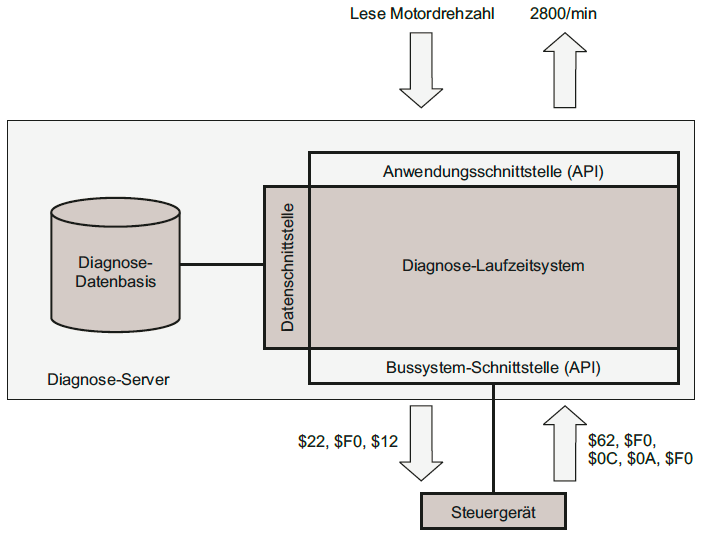
\includegraphics[width=\textwidth]{./Diagnose-Kommunikationsprinzip}
	\caption{ASAM/ISO-Diagnose-Server-Prinzip (Kommunikationsprinzip) [Reif]}
	\label{abb:DiagnoseKommunkationsprinzip}
	\end{figure}
	
\end{comment}





\section{Ergebnisbetrachtung} \label{sec:ErgebnisDiagnose} % Zeitkritisch? Echtzeit? Dauer der Verarbeitung, Wiederholungsrate der Sensorsignale, Rechenleistung, Synchronisation, Berechnung Größe aller Variablen und Summe Bytes der CAN-Frames, Vergleich mit Datenrate CAN um auf Echtzeitfähigkeit zu kommen. Busauslastung? Erst ohne Timing und dann Vorteil von Timing: Unnötige Datenübertragung reduzieren, Busauslastung senken, Mehr Zustandsüberwachungssystem als Diagnosesystem

Wie eingangs erläutert, war es die Intention, eine Diagnosefunktion  vollständig in der ROS-Umgebung einzubinden und als einen neuen Programmknoten umzusetzen, ohne die bereits implementierten Skripte editieren zu müssen. Abbildung \ref{abb:rosgraphMitDiagnose} zeigt, dass dies anhand dem beschriebenen Vorgehen gelungen ist. Der \texttt{diagnostic\_node} reiht sich in dem initialen Programmgraphen ein und hat sämtliche Topics abonniert, die innerhalb ROS publiziert werden. Der Diagnoseknoten selbst veröffentlicht keine Informationen in der Programmumgebung und agiert damit lediglich passiv im ROS-Framework. Die eigentliche Fahrroutine und sämtliche Algorithmen zur Bildverarbeitung und der Fahrzeugregelung werden durch die Diagnosefunktion nicht beeinträchtigt.

\begin{figure}[!htbp]
	\centering
	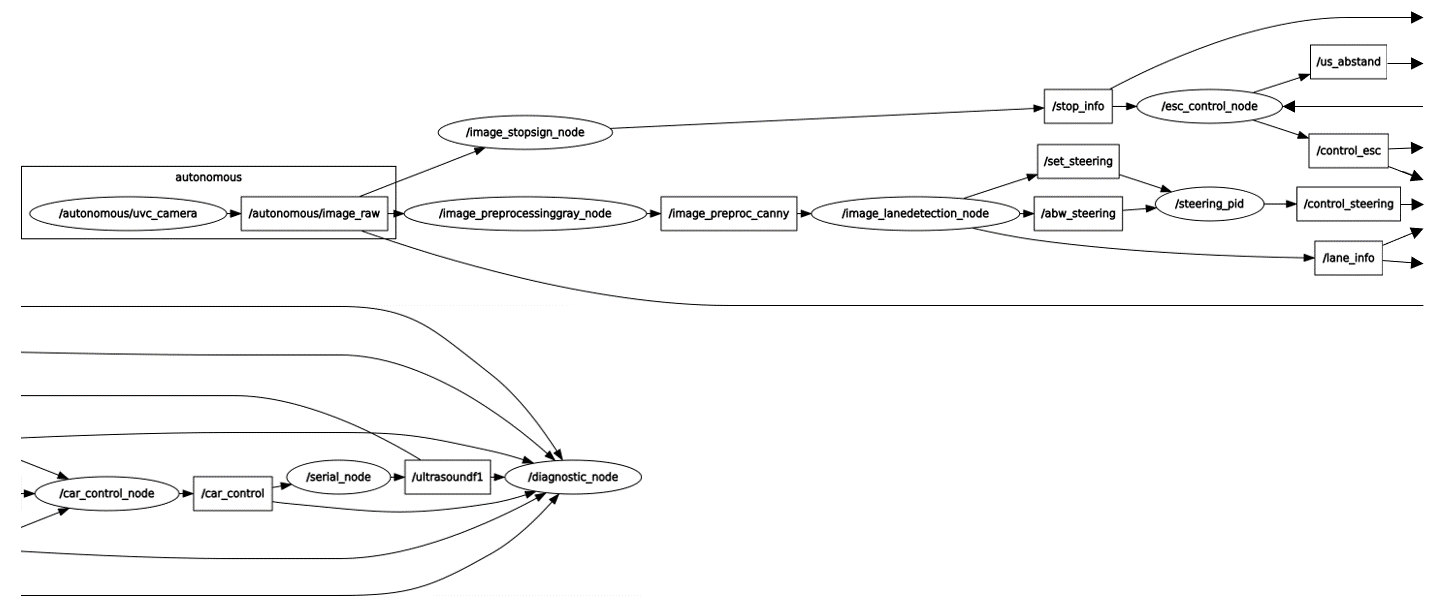
\includegraphics[width=\textwidth]{./rosgraph_mit_diagnose_geteilt}
	\caption{Programmgraph des neuen ROS-Paketes \emph{autonomous} inklusive dem Knoten \emph{diagnostic\_node}, mit dem Befehl \texttt{rqt\_graph} automatisch generiert}
	\label{abb:rosgraphMitDiagnose}
\end{figure} 

\subsection{Test und Validierung} \label{subsec:TestValidierungDiagnose}
\subsection{Mehrwert der Diagnosefunktion} \label{subsec:MehrwertDiagnose}
% Alternative: UDP Das User Datagram Protocol, kurz UDP, ist ein minimales, verbindungsloses Netzwerkprotokoll, das zur Transportschicht der Internetprotokollfamilie gehört. UDP ermöglicht Anwendungen den Versand von Datagrammen in IP-basierten Rechnernetzen. --> Kabellos!



